\section{Herança, encapsulamento e polimorfismo}

\begin{frame}{Herança}
\framesubtitle{}
\begin{itemize}
    \item Criar uma classe derivada a partir de uma classe base
    \item Classe derivada herda os atributos e métodos da base
\end{itemize}
\end{frame}

\begin{frame}{Herança}
\framesubtitle{}
\begin{itemize}
    \item Normalmente os construtores e destrutores não são herdados
    \item Métodos herdados podem ser sobrescritos
    \item Novos métodos e atributos podem ser adicionados
\end{itemize}
\end{frame}

\begin{frame}{Herança}
\framesubtitle{Tipos}
\begin{itemize}
    \item Simples
    \item Múltipla
    \item Multinível
\end{itemize}
\end{frame}

\begin{frame}{Herança}
\framesubtitle{Simples}
\begin{itemize}
    \item Cada classe tem no máximo uma superclasse
    \item A hierarquia pode ser representada por uma árvore
\end{itemize}
\begin{figure}
	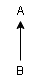
\includegraphics{img/simples}
\end{figure}
\end{frame}

\begin{frame}{Herança}
\framesubtitle{Múltipla}
\begin{itemize}
    \item Cada classe pode ter diversas superclasses
    \item Pode ser necessário tratar ambiguidades na herança
    \item A hierarquia pode ser representada por um grafo direcionado
\end{itemize}
\begin{figure}
	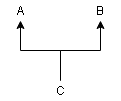
\includegraphics{img/multipla.png}
\end{figure}
\end{frame}

\begin{frame}{Herança}
\framesubtitle{Multinível}
\begin{itemize}
    \item Uma classe derivada pode ser base de outra classe
\end{itemize}
\begin{figure}
	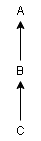
\includegraphics{img/multinivel.png}
\end{figure}
\end{frame}

\begin{frame}{Herança}
\framesubtitle{Usos}
\begin{itemize}
    \item Reuso de código
    \item Implementar uma mesma interface de diferentes formas
\end{itemize}
\end{frame}

\begin{frame}{Encapsulamento}
\framesubtitle{}
\begin{itemize}
    \item Agrupar dados e métodos que agem sobre esses dados
    \item Restringir o acesso direto aos dados
\end{itemize}
\end{frame}

\begin{frame}{Encapsulamento}
\framesubtitle{Usos}
\begin{itemize}
    \item Esconder informação
    \item Esconder detalhes de implementação
    \item Evitar que o objeto entre em um estado inválido
\end{itemize}
\end{frame}

\begin{frame}{Polimorfismo}
\framesubtitle{}
\begin{itemize}
    \item Utilizar o mesmo símbolo para representar vários tipos
    \item Tratar objetos de uma classe derivada com objetos da classe base
\end{itemize}
\end{frame}

\begin{frame}{Polimorfismo}
\framesubtitle{Tipos}
\begin{itemize}
    \item Ad hoc
    \item Paramétrico
    \item Por subtipos
\end{itemize}
\end{frame}

\begin{frame}[fragile]
\frametitle{Polimorfismo}
\framesubtitle{Ad hoc}
\begin{itemize}
    \item Sobrecarga de operador/função
    \item Definir diversas funções com mesmo nome e quantidade de argumentos, mas com diferentes tipos
\end{itemize}
\begin{verbatim}
    soma(a: int, b: int) : int
    soma(a: float, b: float) : float
\end{verbatim}
\end{frame}

\begin{frame}{Polimorfismo}
\framesubtitle{Paramétrico}
\begin{itemize}
    \item Definir funções que aceita um tipo genérico
    \item O comportamento da função é uniforme em relação ao tipo da entrada
\end{itemize}
\end{frame}

\begin{frame}{Polimorfismo}
\framesubtitle{Por subtipos}
\begin{itemize}
    \item Definir uma função que aceita um tipo A
    \item A função funciona corretamente para um subtipo de A
\end{itemize}
\end{frame}